
\section{Results}
\label{sec:results}
% =============================================================================

\subsection{Longitudinal operator learning with FNO}
\label{subsec:results_fno}

\subsubsection{Learning reduced longitudinal profiles}
\label{subsubsec:fno_longitudinal_profiles}

The first experimental block evaluates whether a Fourier Neural Operator can learn a reduced longitudinal map
\begin{equation}
\widehat{\mathcal{T}}_{\theta}
:
(\lambda_{\mathrm{in}},\mu)
\mapsto
\lambda_{\mathrm{out}}.
\label{eq:fno_longitudinal_map_results}
\end{equation}
This task is lower-dimensional than full six-dimensional transport, but remains physically meaningful because longitudinal collective effects are naturally expressed through line densities, wake kernels, and impedance spectra. It also provides a controlled setting in which the operator-learning hypothesis can be tested before moving to the latent six-dimensional problem.

\begin{figure}[htbp]
\centering
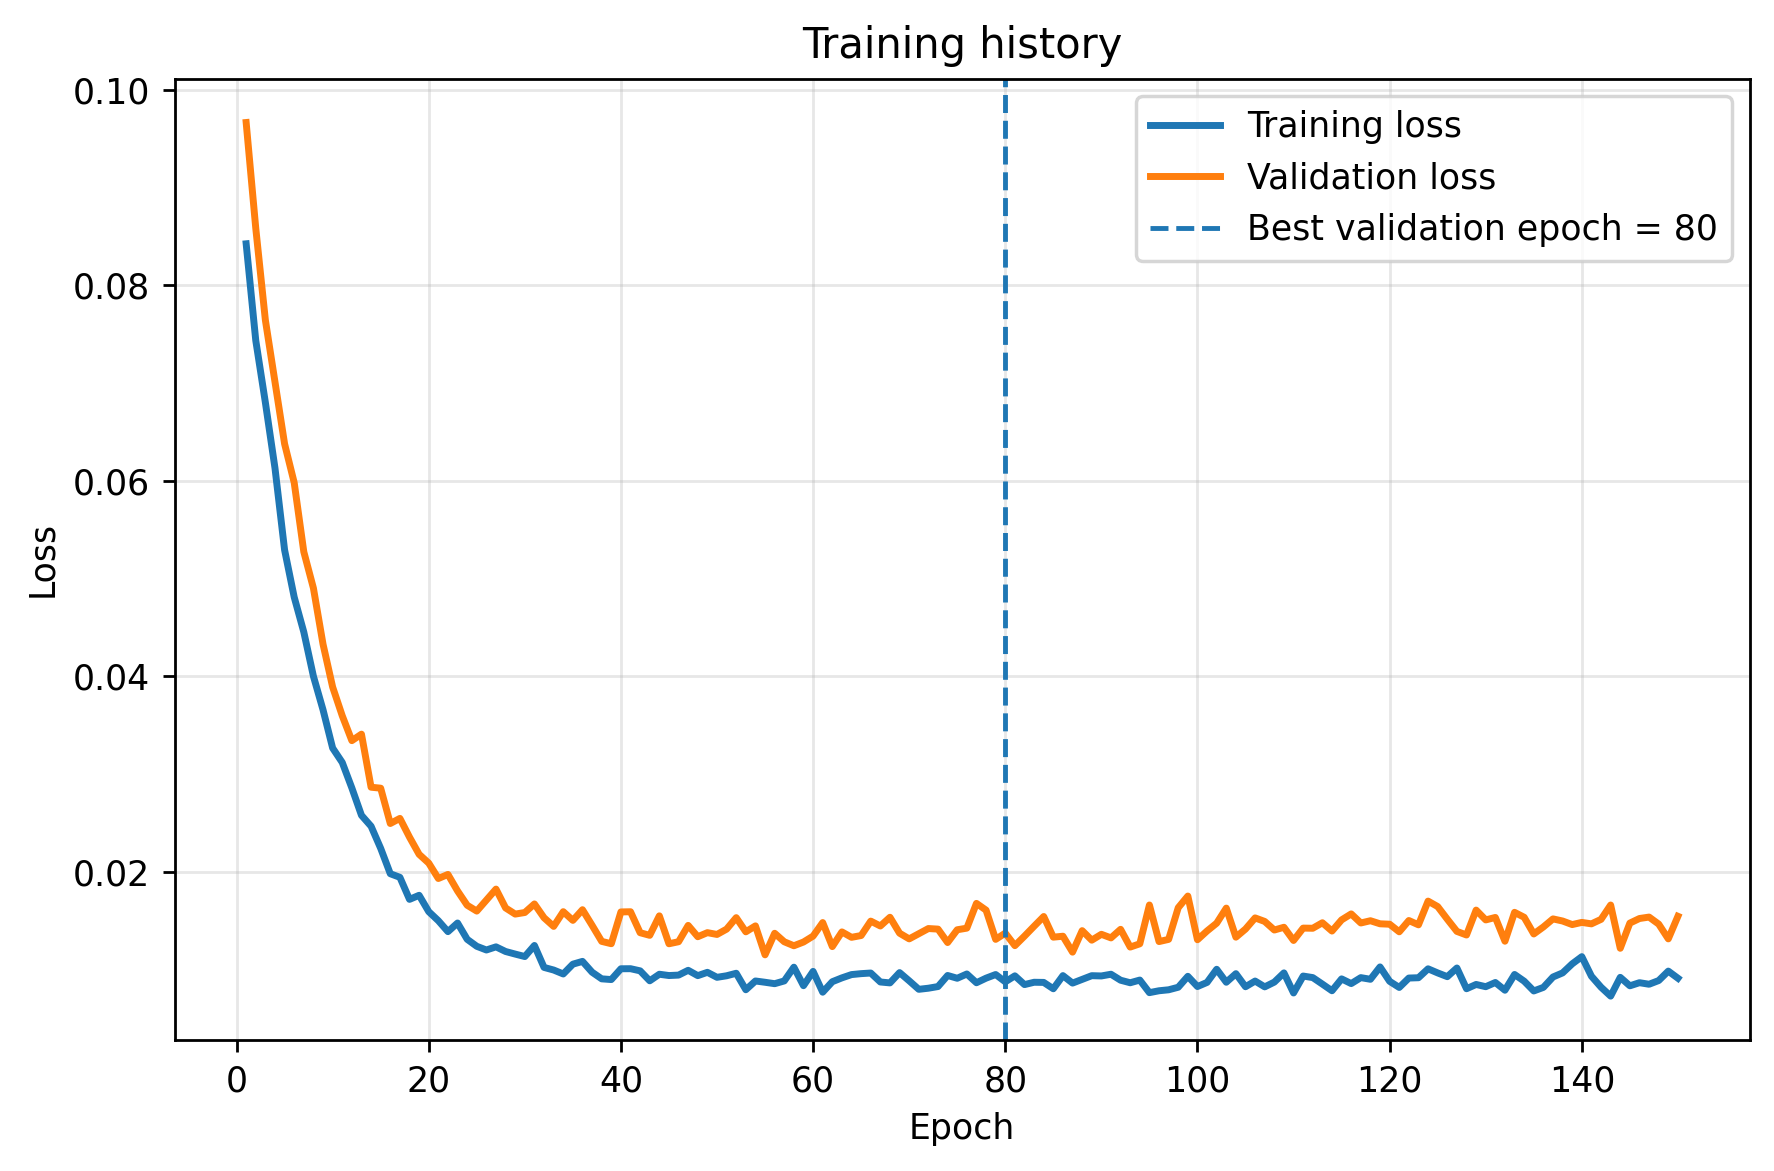
\includegraphics[
width=0.82\textwidth
]{images/results/png/training_history_1d.png}
\caption{
Training and validation loss histories for the one-dimensional FNO longitudinal surrogate. The curves illustrate the convergence of the optimization procedure over the training epochs and the evolution of the model performance on the validation set.
}
\label{fig:fno_1d_training_history}
\end{figure}

\subsubsection{Ha\"issinski-profile reconstruction}
\label{subsubsec:fno_haissinski_results}

For stationary longitudinal problems, the FNO can be used to approximate the equilibrium map
\begin{equation}
(W_{\parallel},I,\mu)
\mapsto
\lambda_h.
\label{eq:fno_haissinski_map_results}
\end{equation}
This formulation is closely connected to the Ha\"issinski equation because the equilibrium profile is determined by a nonlinear self-consistent potential. The relevant validation is therefore not limited to pointwise profile accuracy, but also concerns whether the surrogate reproduces derived physical observables such as centroid shift, bunch lengthening, and peak displacement.

\begin{figure}[h!]
\centering
\safeincludegraphics[width=0.78\textwidth]
{images/generated/training_pycolleff.png}
\caption{
Representative line density reconstruction showed along logarithmic error. The FNO prediction \(\widehat{\lambda}_{\mathrm{out}}\) is compared with the reference profile \(\lambda_{\mathrm{out}}\). The residual representation, \(\widehat{\lambda}_{\mathrm{out}}-\lambda_{\mathrm{out}}\), provides a complementary view of systematic reconstruction error.
}
\label{fig:fno_longitudinal_reconstruction}
\end{figure}

\begin{figure}[h!]
\centering
\safeincludegraphics[width=0.88\textwidth]
{images/generated/line_pred_truth_xsuite.png}
\caption{
Representative test-set prediction for the reduced FNO longitudinal surrogate. Randomized noise is added to the sample to illustrate the robustness of the learned operator. The figure compares the reference line density \(\lambda_{\mathrm{out}}\) with the FNO prediction \(\widehat{\lambda}_{\mathrm{out}}\) and the residual field \(\widehat{\lambda}_{\mathrm{out}}-\lambda_{\mathrm{out}}\).
}
\label{fig:fno_profile_predictions_revised}
\end{figure}


% \begin{table}[H]
% \centering
% \caption{
% Quantitative evaluation of the FNO longitudinal surrogate. Replace the placeholders with final test-set values.
% }
% \label{tab:fno_longitudinal_metrics}
% \begin{tabular}{lccc}
% \toprule
% Metric & Mean & Std.\ dev. & Worst case \\
% \midrule
% Relative $L^2$ profile error & --- & --- & --- \\
% Centroid error & --- & --- & --- \\
% Bunch-length error & --- & --- & --- \\
% Peak-position error & --- & --- & --- \\
% Wasserstein distance & --- & --- & --- \\
% Inference time per sample & --- & --- & --- \\
% \bottomrule
% \end{tabular}
% \end{table}

% \subsubsection{Interpretation}
% \label{subsubsec:fno_interpretation}

% The FNO results support the formulation of longitudinal collective effects as operator-learning problems. This interpretation is consistent with the structure of the wake convolution and the spectral representation of impedance. Nevertheless, the FNO also presents limitations. Its formulation is particularly natural on regular grids and for reduced one-dimensional or low-dimensional functional data. Extending the same direct-grid strategy to a complete six-dimensional phase-space density would be computationally prohibitive. The full beam-distribution problem is therefore addressed through a reduced latent representation.

% =============================================================================
\subsection{Six-dimensional latent representation}
\label{subsec:results_latent_representation}
% =============================================================================

\subsubsection{CVAE reconstruction quality}
\label{subsubsec:cvae_reconstruction_quality}

The next experimental block evaluates whether the fifteen-projection representation can be compressed into a latent variable while preserving physically relevant structure of the beam distribution. The CVAE reconstructs the projected histograms from a latent state \(z\) and conditioning variables \(c\), while auxiliary physical information may be treated through explicit conditioning or a dedicated physical-dimensions head.

\begin{figure}[htbp]
\centering
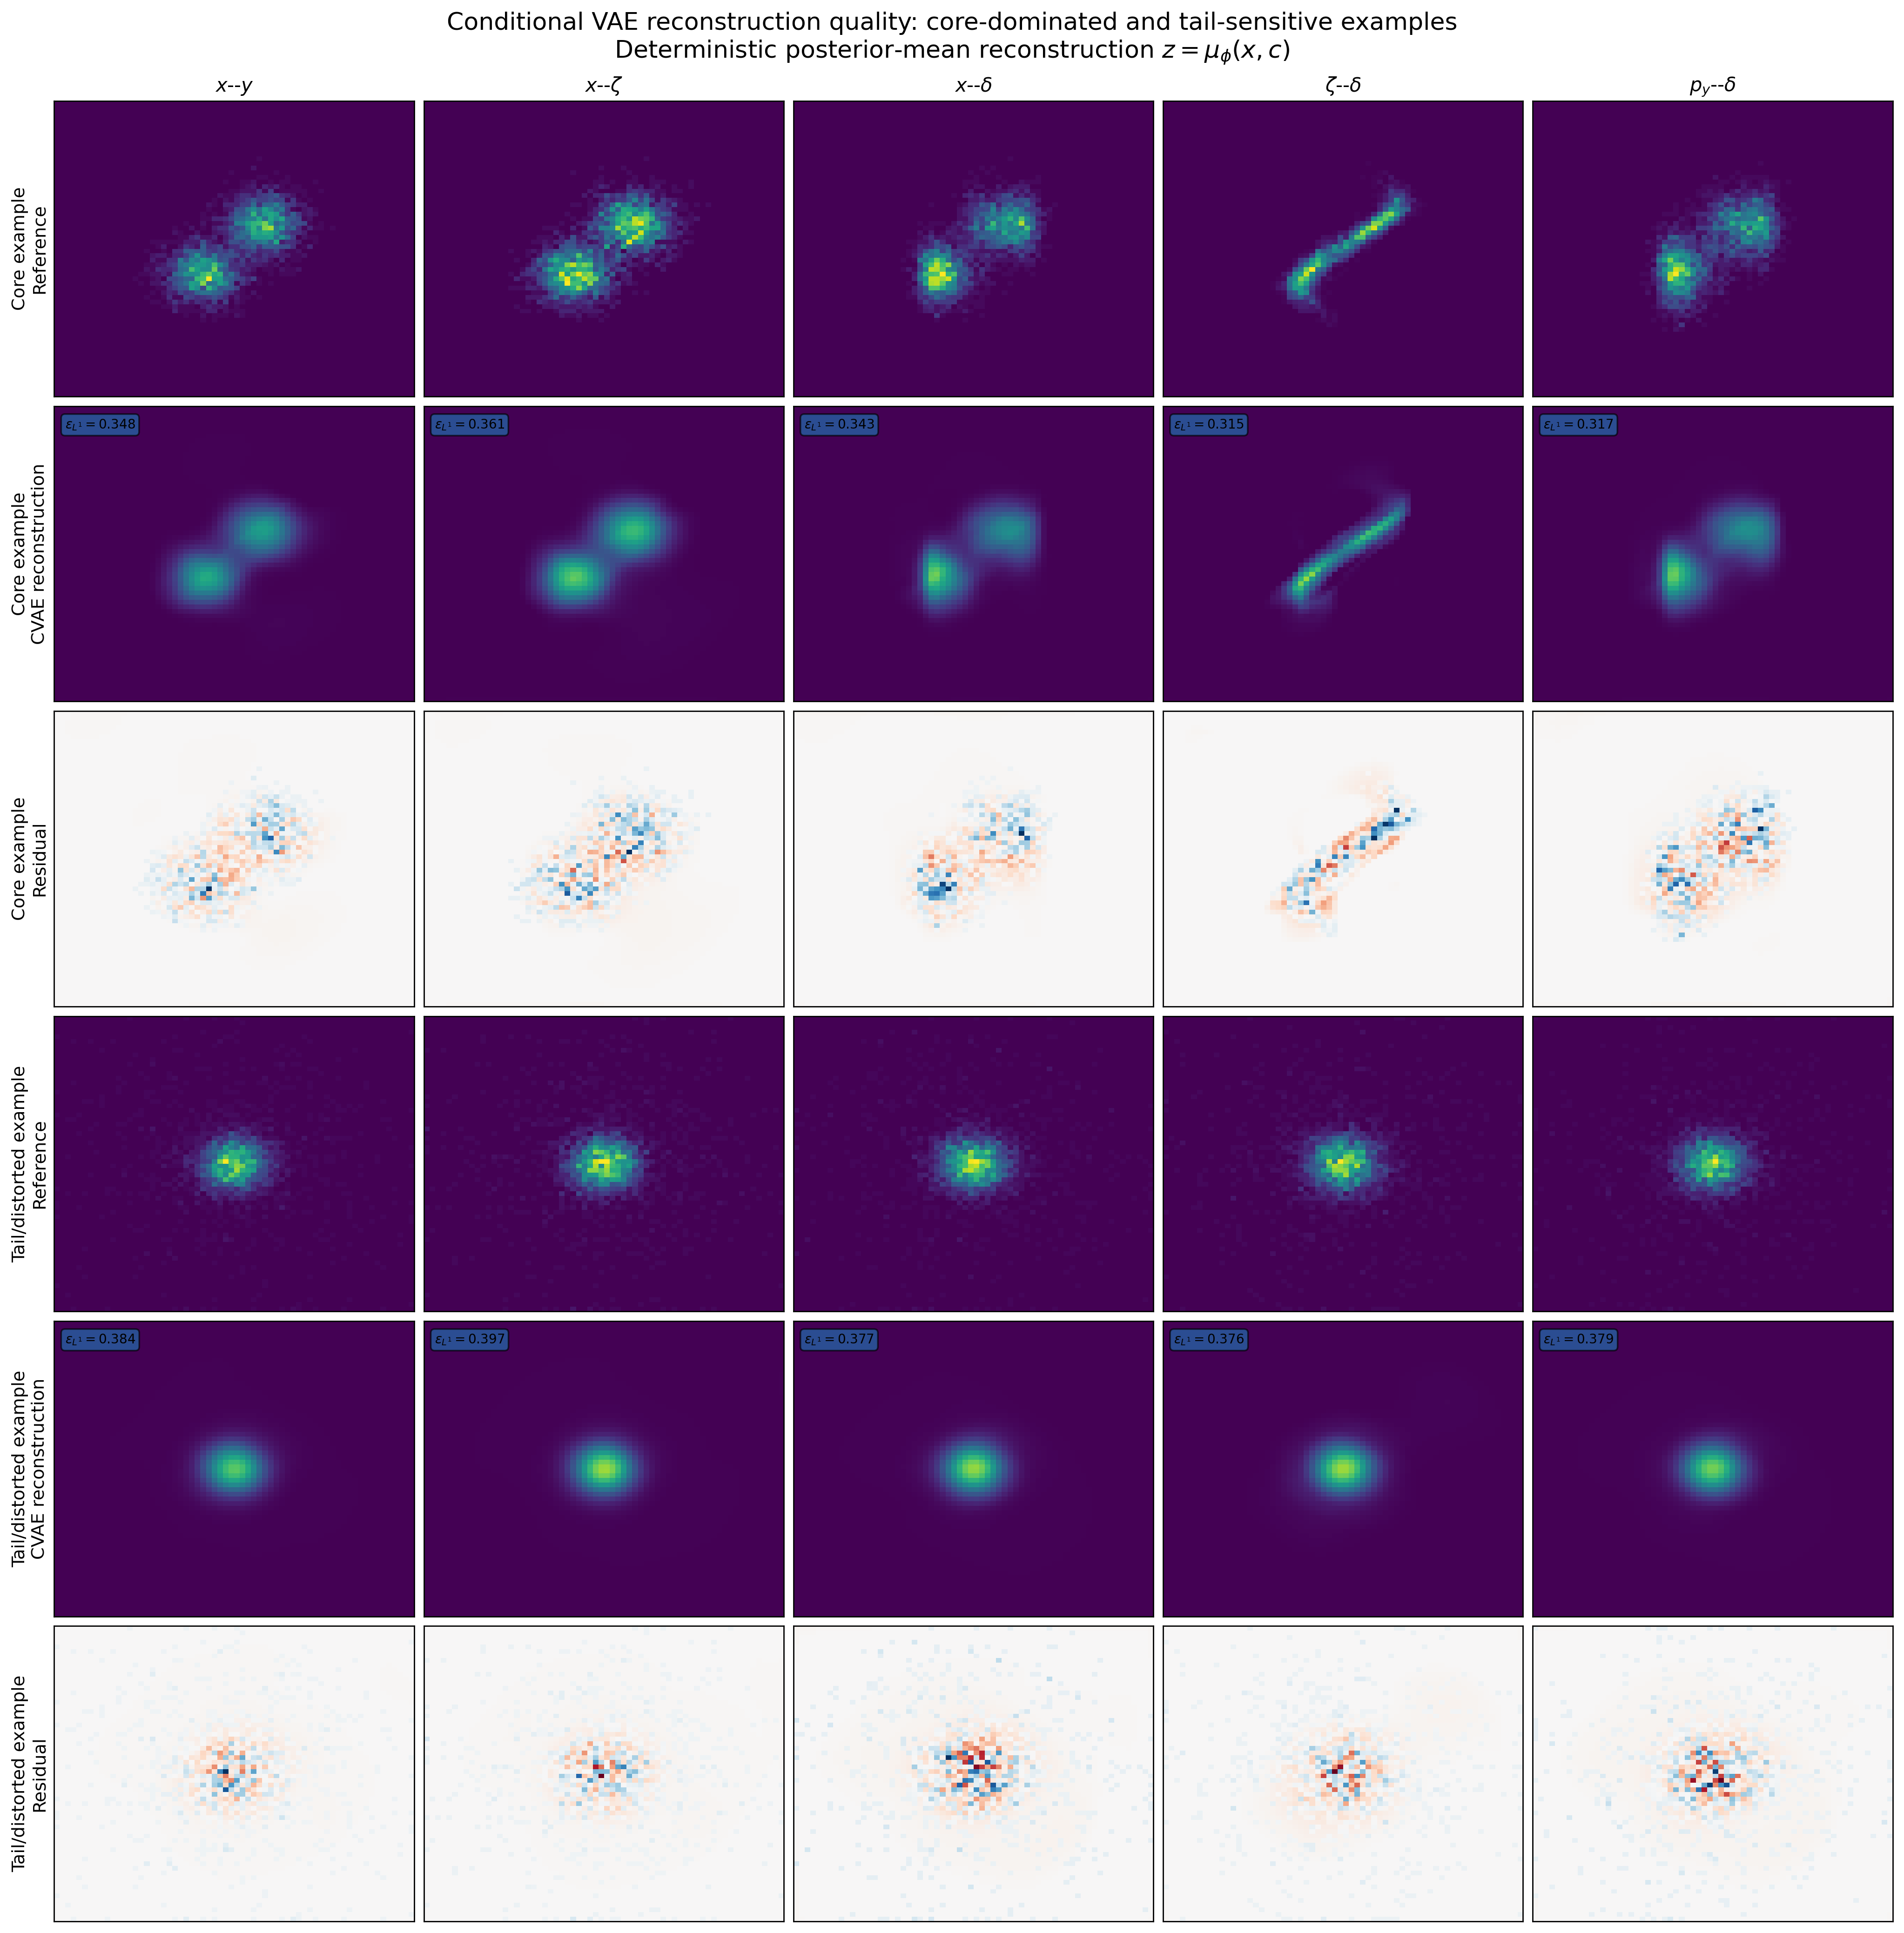
\includegraphics[
width=0.98\textwidth
]{images/results/png/cvae_reconstruction_quality.png}
\caption{
Conditional VAE reconstruction quality for representative beam distributions. The comparison illustrates both the fidelity of the reconstructed high-density core and the increased difficulty associated with lower-density tails and distorted phase-space structure.
}
\label{fig:cvae_reconstruction_quality}
\end{figure}

\begin{table}[H]
\centering
\caption{
Quantitative CVAE reconstruction metrics. 
}
\label{tab:cvae_reconstruction_metrics}
\begin{tabular}{lccc}
\toprule
Metric & Train & Validation & Test \\
\midrule
Histogram relative error & 0.362 & 0.357 & 0.367 \\
Moment error & 0.178 & 0.243 & 0.264 \\
KL term & 929.275 & 921.513 & 920.925 \\
Sliced Wasserstein distance & 0.0092 & 0.0089 & 0.0096 \\
\bottomrule
\end{tabular}

\end{table}

\subsubsection{Latent-space diagnostics}
\label{subsubsec:latent_space_diagnostics}

A well-regularized latent space should not simply memorize the training samples. To investigate this point, the latent coordinates are compared with physically interpretable observables. In the present work, Pearson correlations are evaluated between the latent variables and beam statistics including coordinate means and RMS spread extensions. For a physical observable \(q\) and latent coordinate \(z_k\), the Pearson correlation coefficient is
\begin{equation}
r_{q,z_k}
=
\frac{
\operatorname{Cov}(q,z_k)
}{
\sigma_q \sigma_{z_k}
}.
\label{eq:pearson_latent_physics}
\end{equation}

For each physical observable, the twenty latent coordinates with the largest absolute correlations can be displayed,
\begin{equation}
\left\{
z_{k_1},
\ldots,
z_{k_{20}}
\right\}
=
\operatorname{TopK}_{20}
\left(
|r_{q,z_k}|
\right).
\label{eq:top20_latent_correlations}
\end{equation}

\begin{figure}[htbp]
    \centering
    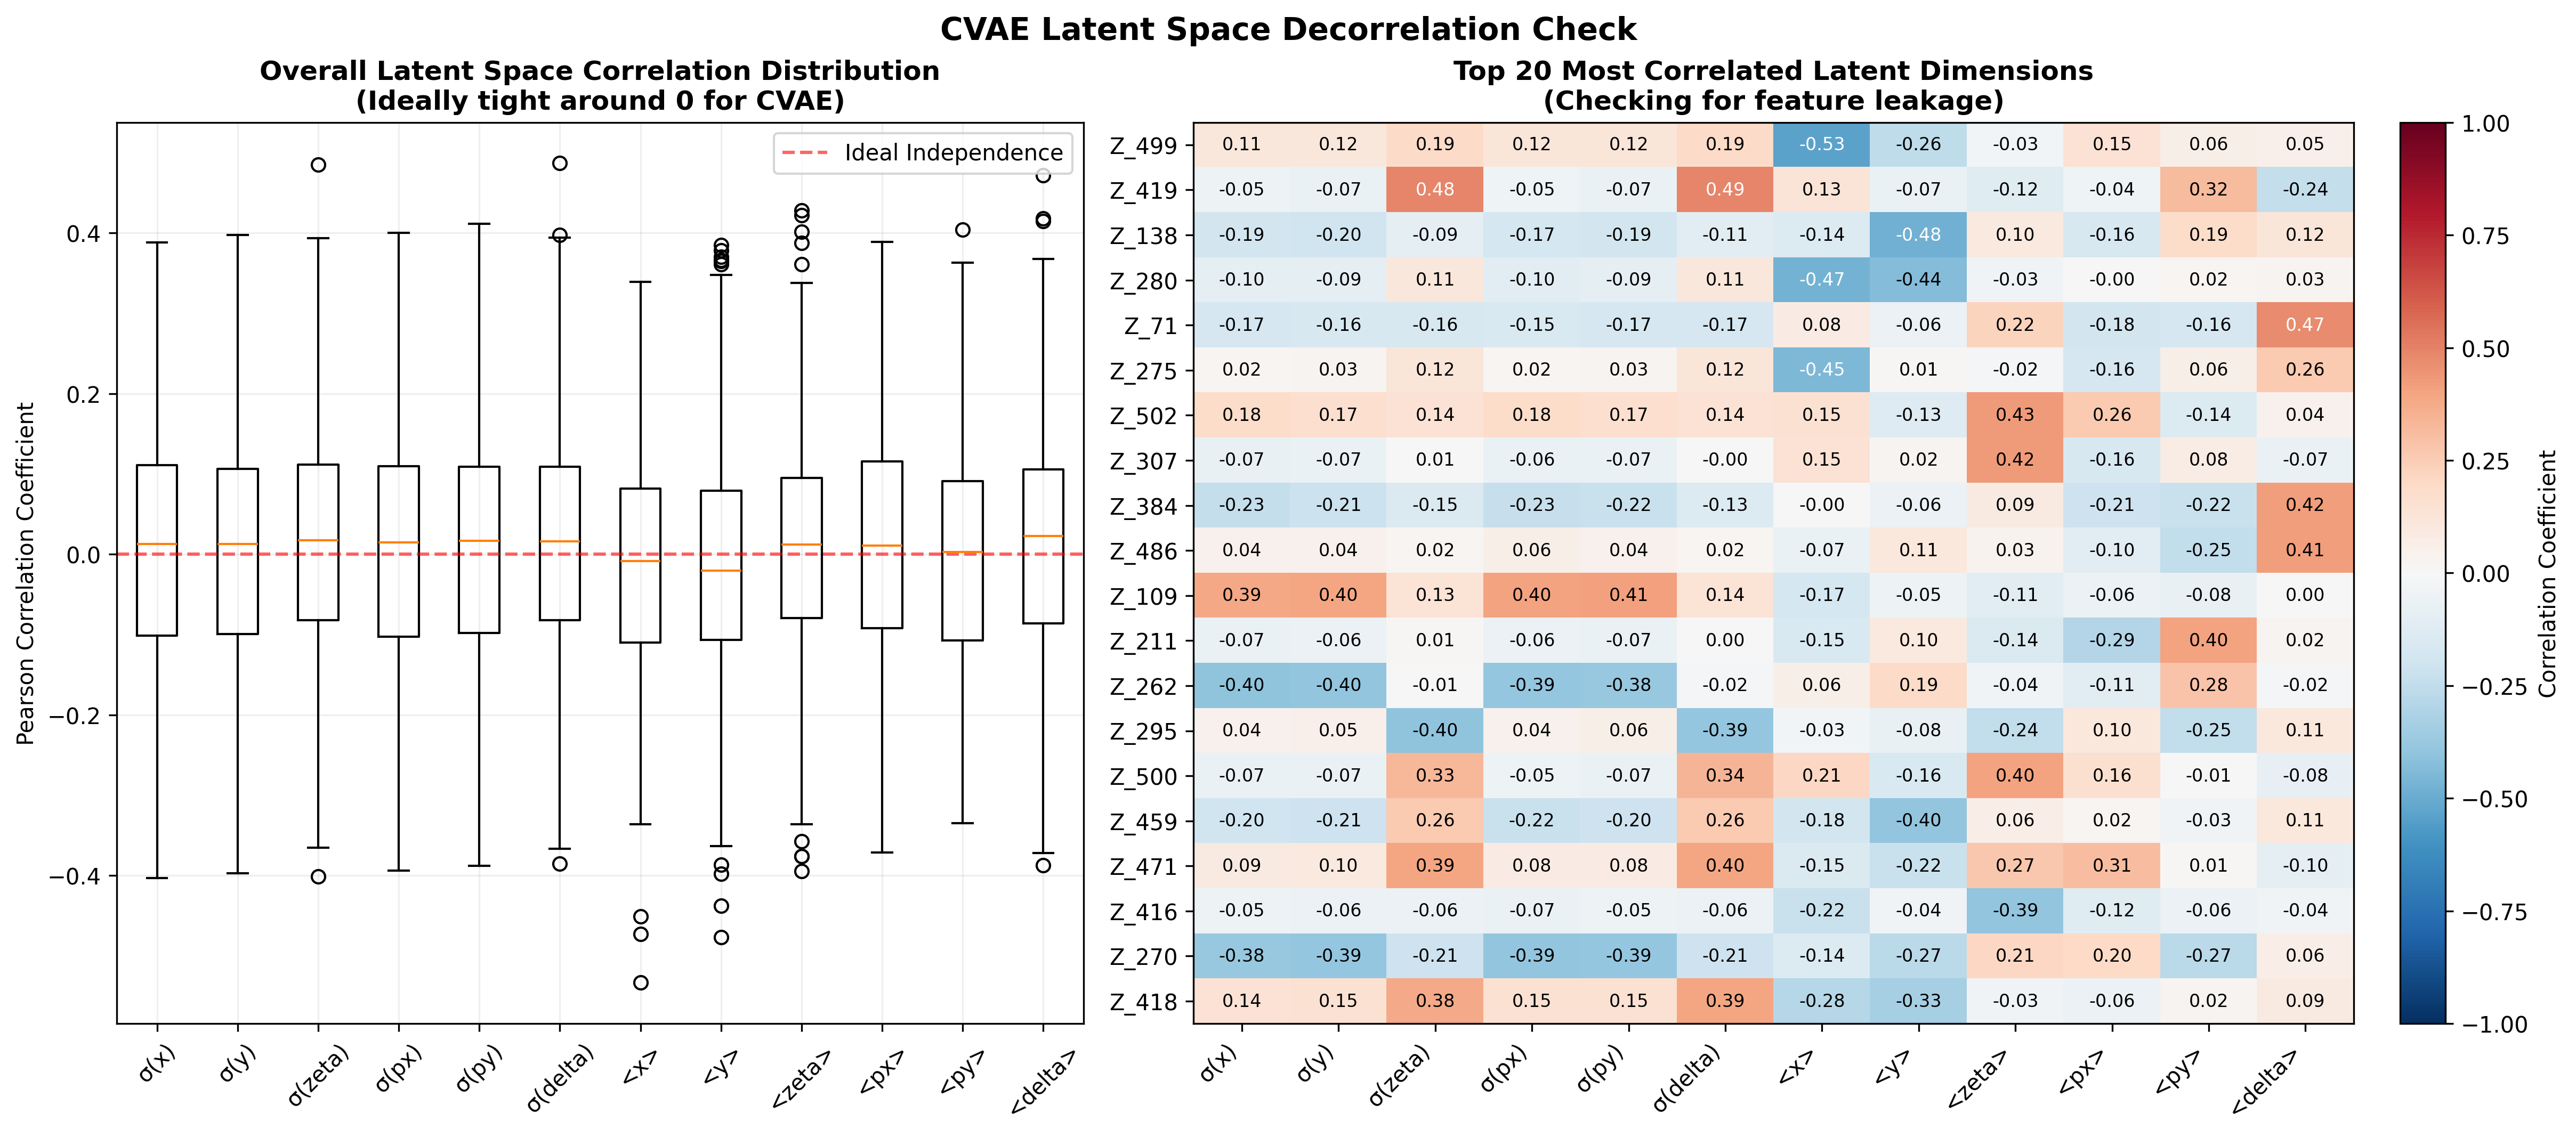
\includegraphics[
        width=\textwidth,
        keepaspectratio
    ]{images/results/png/correlation_CVAE.png}
    \caption{
        Pearson-correlation diagnostics between the CVAE latent representation
        and the auxiliary physical beam statistics. The left panel shows the
        distribution of signed correlation coefficients across the
        $512$ latent coordinates for each of the $12$ physical observables,
        comprising the six coordinate-wise rms spreads
        $\boldsymbol{\sigma}
        =(\sigma_x,\sigma_y,\sigma_\zeta,\sigma_{p_x},
        \sigma_{p_y},\sigma_\delta)$
        and the six phase-space centroids
        $\langle\mathbf{x}\rangle
        =(\langle x\rangle,\langle y\rangle,\langle\zeta\rangle,
        \langle p_x\rangle,\langle p_y\rangle,\langle\delta\rangle)$.
        The right panel displays the full correlation patterns of the
        $20$ latent coordinates attaining the largest absolute correlation
        with any physical observable. The signed distributions remain
        concentrated around zero and no single physical statistic produces
        a systematic displacement of the latent population.
    }
    \label{fig:cvae_latent_correlation}
\end{figure}

To quantify the behavior shown in
Fig.~\ref{fig:cvae_latent_correlation}, Pearson coefficients were
computed between every latent coordinate and every auxiliary physical
observable over the validation subset. With $N_{\mathrm{val}}=51$
samples, a latent dimension $d_z=512$, and $12$ physical observables,
the diagnostic contains $512\times 12 = 6144$ pairwise correlation coefficients. The corresponding global statistics are summarized in Table~\ref{tab:cvae_global_correlation}.

\begin{table}[htbp]
    \centering
    \caption{
        Global latent--physical Pearson-correlation statistics for the CVAE.
        The threshold counts refer to the full set of $6144$ latent--physical
        pairs.
    }
    \label{tab:cvae_global_correlation}
    \begin{tabular}{lcc}
        \toprule
        Diagnostic & Value & Fraction of pairs \\
        \midrule
        Mean absolute correlation
            & $0.1161$ & -- \\
        Median absolute correlation
            & $0.1006$ & -- \\
        Standard deviation of $|r|$
            & $0.0846$ & -- \\
        Maximum absolute correlation
            & $0.5333$ & -- \\
        $|r|\geq 0.20$
            & $1031/6144$ & $16.78\%$ \\
        $|r|\geq 0.30$
            & $198/6144$ & $3.22\%$ \\
        $|r|\geq 0.40$
            & $18/6144$ & $0.29\%$ \\
        $|r|\geq 0.50$
            & $1/6144$ & $0.016\%$ \\
        \bottomrule
    \end{tabular}
\end{table}

The global correlation distribution is tightly concentrated around
zero. In particular, the mean and median absolute coefficients are
$0.1161$ and $0.1006$, respectively, while only $18$ of the $6144$
tested pairs exceed $|r|=0.4$ and only one exceeds $|r|=0.5$.
The largest individual coefficient,
\[
    r\!\left(z_{499},\langle x\rangle\right)=-0.5333,
\]
should therefore be interpreted in the context of both the limited
validation sample size and the simultaneous inspection of several
thousand latent--physical pairs. An isolated extreme coefficient is
not, by itself, evidence that a physical observable is systematically
encoded throughout the latent representation.

This interpretation is further supported by the observable-wise
statistics in Table~\ref{tab:cvae_feature_correlation}. The mean
absolute correlation remains within the narrow interval
\[
    0.1098
    \leq
    \frac{1}{d_z}
    \sum_{j=1}^{d_z}
    \left|
        r(z_j,a_k)
    \right|
    \leq
    0.1203
\]
for every physical observable $a_k$. Consequently, no individual beam
size or centroid produces a globally enhanced response across the
latent coordinates.

\begin{table}[htbp]
    \centering
    \caption{
        Observable-wise Pearson-correlation summary on the validation set. For each physical statistic, the table reports the mean and median absolute Pearson correlation over all $512$ latent coordinates, together with the strongest individual signed coefficient. These statistics quantify linear association only and do not test general nonlinear dependence.
    }
    \label{tab:cvae_feature_correlation}
    \small
    \begin{tabular}{lcccc}
        \toprule
        Observable
        & Mean $|r|$
        & Median $|r|$
        & Max. $|r|$
        & Strongest pair \\
        \midrule
        $\sigma_x$
            & $0.1203$ & $0.1078$ & $0.4030$
            & $r(z_{262},\sigma_x)=-0.4030$ \\
        $\sigma_y$
            & $0.1199$ & $0.1047$ & $0.3974$
            & $r(z_{262},\sigma_y)=-0.3974$ \\
        $\sigma_\zeta$
            & $0.1174$ & $0.1013$ & $0.4849$
            & $r(z_{419},\sigma_\zeta)=+0.4849$ \\
        $\sigma_{p_x}$
            & $0.1200$ & $0.1062$ & $0.4002$
            & $r(z_{109},\sigma_{p_x})=+0.4002$ \\
        $\sigma_{p_y}$
            & $0.1201$ & $0.1052$ & $0.4112$
            & $r(z_{109},\sigma_{p_y})=+0.4112$ \\
        $\sigma_\delta$
            & $0.1172$ & $0.0981$ & $0.4867$
            & $r(z_{419},\sigma_\delta)=+0.4867$ \\
        $\langle x\rangle$
            & $0.1157$ & $0.1003$ & $0.5333$
            & $r(z_{499},\langle x\rangle)=-0.5333$ \\
        $\langle y\rangle$
            & $0.1170$ & $0.0934$ & $0.4767$
            & $r(z_{138},\langle y\rangle)=-0.4767$ \\
        $\langle\zeta\rangle$
            & $0.1098$ & $0.0861$ & $0.4278$
            & $r(z_{502},\langle\zeta\rangle)=+0.4278$ \\
        $\langle p_x\rangle$
            & $0.1143$ & $0.1023$ & $0.3891$
            & $r(z_{381},\langle p_x\rangle)=+0.3891$ \\
        $\langle p_y\rangle$
            & $0.1107$ & $0.0994$ & $0.4038$
            & $r(z_{211},\langle p_y\rangle)=+0.4038$ \\
        $\langle\delta\rangle$
            & $0.1114$ & $0.0954$ & $0.4716$
            & $r(z_{71},\langle\delta\rangle)=+0.4716$ \\
        \bottomrule
    \end{tabular}
\end{table}

The strongest Pearson coefficients do not reveal a single physical observable that is uniformly aligned with the latent representation. Instead, the largest coefficients involve different transverse and longitudinal centroids and coordinate-wise RMS spreads, and are distributed across several latent coordinates. For example, the strongest individual associations involve $\langle x\rangle$, $\sigma_\delta$, $\langle y\rangle$, $\langle\delta\rangle$, $\langle\zeta\rangle$, and $\sigma_{p_y}$. This heterogeneity indicates that the largest observed linear associations are not concentrated on one physical statistic or one latent coordinate. Most importantly, Pearson correlation measures linear association only and therefore cannot rule out nonlinear dependence. The present result should therefore be interpreted only as evidence against a simple, pervasive linear alignment, not as proof of statistical independence or of nonlinear disentanglement.

Overall, the diagnostic provides no evidence of systematic linear leakage of the explicitly supplied beam sizes and centroids into the CVAE latent representation at the resolution allowed by the present validation sample. The result should nevertheless be interpreted as a test of linear dependence rather than a proof of full statistical independence as Pearson coefficients do not exclude nonlinear dependence, and the relatively small value
$N_{\mathrm{val}}=51$ limits the precision of individual correlation estimates. Within these limitations, the observed concentration around zero supports the intended separation between the latent morphological representation and the explicit physical beam statistics.

This result is compatible with the intended role of the CVAE latent representation. The latent coordinates are not required to coincide individually with specific physical observables. Rather, they are expected to provide a distributed reduced representation of the projected density structure. The fact that only a limited subset of latent coordinates carries moderate information about individual observables suggests sparse physical alignment rather than a trivially encoded hidden parameterization.

Complete disentanglement is neither expected nor necessarily desirable. The relevant question is whether the latent state preserves the dynamical degrees of freedom required for propagation while avoiding excessive leakage of scale and position information that can be handled explicitly through physical conditioning variables or the auxiliary physical-dimensions head.

% =============================================================================
\subsection{Transformer latent propagation and the effect of locality}
\label{subsec:results_transformer_locality}
% =============================================================================

\subsubsection{Global-attention baseline}
\label{subsubsec:results_nowindow_transformer}

The first sequence-model baseline investigates whether an expressive Transformer can propagate the CVAE latent representation through the ordered lattice description. In this formulation, the causal mask prevents future or downstream tokens from influencing earlier positions, thereby enforcing upstream-to-downstream information flow. A global causal mask does not, however, impose finite interaction support: the state associated with a given position may, in principle, aggregate information from every preceding token.

This distinction is relevant because the beam state results from an ordered composition of lattice transformations. Although long-range dependence may be physically meaningful, unrestricted upstream mixing can introduce an architectural bias that differs from a predominantly local composition of element-wise transport. The no-window Transformer diagnostics provide a qualitative illustration of this effect.

Let \(H_{ij}\) denote a reference two-dimensional marginal and
\(\widehat{H}_{ij}\) its prediction. The residual field is
\begin{equation}
\varepsilon_{ij}(u,v)
=
\widehat{H}_{ij}(u,v)
-
H_{ij}(u,v).
\label{eq:histogram_residual_field}
\end{equation}
A systematic reconstruction artifact corresponds to a nonzero mean residual
\begin{equation}
b_{ij}(u,v)
=
\mathbb{E}
\left[
\varepsilon_{ij}(u,v)
\right]
\neq 0.
\label{eq:residual_bias_revised}
\end{equation}

At the latent level, an accumulated error mechanism can be represented schematically as
\begin{equation}
z_{n+1}
=
z_n
+
\Delta z_n^{\mathrm{true}}
+
\eta_{\theta,n},
\end{equation}
which gives, after \(N\) propagation steps,
\begin{equation}
z_N
=
z_0
+
\sum_{n=0}^{N-1}
\Delta z_n^{\mathrm{true}}
+
\sum_{n=0}^{N-1}
\eta_{\theta,n}.
\label{eq:latent_error_accumulation}
\end{equation}
If the learned local error has a systematic component,
\begin{equation}
\mathbb{E}
\left[
\eta_{\theta,n}
\right]
\neq 0,
\end{equation}
the decoded rollout can develop a coherent distortion rather than a zero-centered random error. This mechanism does not prove that unrestricted attention is uniquely responsible for the observed artifacts. It nevertheless motivates the controlled locality study introduced next.

\subsubsection{Local-window Transformer}
\label{subsubsec:results_window_transformer}

To test whether unrestricted upstream mixing contributes to the observed reconstruction error, the Transformer attention support is restricted through the local causal mask introduced in Eq.~\eqref{eq:window_mask_revised}. In the principal Transformer--GNO comparison presented below, the Transformer implementation uses an attention window $w=8$. Thus, the hidden state at sequence position \(i\) can only aggregate information from a finite upstream neighborhood.

The effect of this restriction is evaluated first through the longitudinal marginal $(\zeta,\delta)$, which is particularly sensitive to the local correlation structure of the beam. The conditional-slice diagnostic introduced in Section~\ref{subsubsec:results_nowindow_transformer} is applied to the local-window Transformer reconstruction. This marginal is central in the study of longitudinal collective effects, which are the primary physical motivation for the present work.

\begin{figure}[h!]
\centering
\safeincludegraphics[width=0.94\textwidth]
{images/results/png/TF_conditionals_longitudinal.png}
\caption{
Conditional-slice consistency of the local-window Transformer for the longitudinal \((\zeta,\delta)\) marginal. The diagnostic compares predicted and reference conditional means for constant-\(\zeta\) and constant-\(\delta\) slices. Error bars encode local conditional spread. Concentration around the ideal parity relation indicates preservation of internal longitudinal phase-space structure beyond agreement of global moments.
}
\label{fig:tf_conditionals_longitudinal}
\end{figure}

The local-window result is important because the architectural modification does not change the underlying CVAE representation or the physical prediction target. Instead, it changes the support of the interaction mechanism used during latent propagation. The resulting comparison therefore isolates, to first order, the role of locality as an inductive bias.

% =============================================================================
\subsection{CVAE with Graph Neural Operator propagation}
\label{subsec:results_cvae_gno}
% =============================================================================

\subsubsection{Consistency in longitudinal dynamics}
\label{subsubsec:gno_longitudinal_conditionals}

The Graph Neural Operator provides the second latent propagation mechanism. In contrast with attention-based sequence mixing, the GNO represents information transfer through a learned kernel evaluated over the graph neighborhood introduced in Section~\ref{subsec:graph_neural_operator}. The same longitudinal conditional diagnostic is applied to the GNO reconstruction.

\begin{figure}[h!]
\centering
\safeincludegraphics[width=0.94\textwidth]
{images/results/png/GNO_conditionals_longitudinal.png}
\caption{
Conditional-slice consistency of the CVAE--GNO surrogate for the longitudinal \((\zeta,\delta)\) marginal. The figure evaluates agreement of local conditional means under constant-\(\zeta\) and constant-\(\delta\) slicing. Comparison with Fig.~\ref{fig:tf_conditionals_longitudinal} isolates differences in internal phase-space reconstruction between local-window attention and graph-kernel propagation.
}
\label{fig:gno_conditionals_longitudinal}
\end{figure}

The conditional analysis complements global histogram errors. Two models may attain similar integrated reconstruction losses while distributing their residuals differently across the support of the beam. Conditional means therefore provide a direct probe of whether correlations between longitudinal position and energy deviation are preserved locally.

% =============================================================================
\subsection{Direct comparison of local-window Transformer and GNO}
\label{subsec:results_tf_gno_comparison}
% =============================================================================

\subsubsection{Two-dimensional marginal reconstruction}
\label{subsubsec:results_tf_gno_marginals}

A direct comparison is performed on the same selected sample, $s=3$, used in the previous conditional diagnostics. The sample is evaluated at the same four representative pairwise phase-space projections, which are displayed in Figs.~\ref{fig:tf_gno_comparison_xy_xzeta} and \ref{fig:tf_gno_comparison_xdelta_longitudinal}. The comparison is performed at the histogram level, with residuals defined as   

The residuals are evaluated as
\begin{equation}
\Delta H_{\mathrm{TF}}
=
\widehat{H}_{\mathrm{TF}}-H,
\qquad
\Delta H_{\mathrm{GNO}}
=
\widehat{H}_{\mathrm{GNO}}-H.
\label{eq:tf_gno_density_residuals}
\end{equation}

\begin{figure}[p]
\centering
\safeincludegraphics[width=0.96\textwidth]
{images/results/png/comparison_s3_p0_x_y.png}


\vspace{0.8em}

\safeincludegraphics[width=0.96\textwidth]
{images/results/png/comparison_s3_p1_x_zeta.png}

\caption{
Direct density-level comparison of the local-window Transformer and GNO for sample \(s=3\). Top: transverse cross-plane marginal \((x,y)\), pair \(p=0\). Bottom: mixed transverse--longitudinal marginal \((x,\zeta)\), pair \(p=1\). Each row displays the reference density, both model predictions, and their residual fields.
}
\label{fig:tf_gno_comparison_xy_xzeta}


\end{figure}

\begin{figure}[p]
\centering
\safeincludegraphics[width=0.96\textwidth]
{images/results/png/comparison_s3_p4_x_delta.png}


\vspace{0.8em}

\safeincludegraphics[width=0.96\textwidth]
{images/results/png/comparison_s3_p11_zeta_delta.png}

\caption{
Direct density-level comparison of the local-window Transformer and GNO for sample \(s=3\). Top: mixed transverse--energy marginal \((x,\delta)\), pair \(p=4\). Bottom: longitudinal phase-space marginal \((\zeta,\delta)\), pair \(p=11\). The common residual representation exposes structured model error that may be obscured by scalar reconstruction metrics.
}
\label{fig:tf_gno_comparison_xdelta_longitudinal}


\end{figure}

The selected marginals probe complementary structures. The \((x,y)\) distribution tests coupling between transverse coordinates; \((x,\zeta)\) and \((x,\delta)\) probe mixed correlations between transverse and longitudinal degrees of freedom; and \((\zeta,\delta)\) directly tests reconstruction of longitudinal phase-space structure. Consequently, agreement across these projections provides a stronger diagnostic than evaluation of a single preferred plane.

Qualitatively, the comparison should be interpreted through both residual amplitude and residual organization. A model may exhibit a moderate pointwise error while remaining approximately unbiased, whereas coherent positive and negative residual lobes reveal systematic deformation of the predicted distribution. The latter is particularly relevant when evaluating whether the surrogate preserves the location, orientation, and extension of phase-space structures.

The selected marginals probe complementary structures. The $(x,y)$ distribution tests coupling between transverse coordinates, $(x,\zeta)$ and $(x,\delta)$ probe mixed transverse--longitudinal correlation, and $(\zeta,\delta)$  directly tests reconstruction of longitudinal phase-space structure. Agreement across these projections therefore provides a more informative qualitative diagnostic than evaluation on a single preferred plane. 

Both the local-window Transformer and the CVAE--GNO reproduce the main location, orientation, and spatial extension of the distributions in the examples shown. On the basis of these selected marginals alone, neither model can be declared systematically superior. The comparison should instead distinguish between residual amplitude and residual organization. A model may exhibit moderate pointwise error while remaining approximately unbiased, whereas coherent positive and negative residual lobes indicate a systematic deformation of the reconstructed density.

A quantitative distinction between the two propagators therefore requires evaluation over the complete held-out test set rather than visual inspection of individual examples. The relevant criteria include binwise reconstruction error, transport-based discrepancy, systematic bias, and end-to-end inference time. These quantities are compared globally in Table~\ref{tab:global_model_comparison}. Under the reported evaluation conditions, the CVAE--GNO provides the lower aggregate distributional errors, the lower measured bias norm, and the shorter inference time, whereas the local-window Transformer remains competitive in its reconstruction of individual marginals. Robustness to perturbations, changes in lattice configuration, or out-of-distribution parameters is not established by the present comparison and would require a dedicated study.


\subsubsection{Macroparticle-based distributional diagnostics}
\label{subsubsec:results_macroparticle_comparison}

Histogram residuals are complemented by a macroparticle-based analysis. Each predicted two-dimensional density is interpreted as a discrete probability distribution and sampled to generate a large synthetic particle ensemble. In the implemented diagnostic, $N_{\mathrm{sample}}$ macroparticles are drawn from each of the reference, Transformer, and GNO distributions. 

The sampled particle coordinates are transformed back to the corresponding physical range using the reference cloud bounds. Sorted coordinate samples are then compared directly. For a coordinate \(q\), the residuals are
\begin{equation}
r_{\mathrm{TF}}^{(q)}
=
q_{\mathrm{TF}}
-
q_{\mathrm{truth}},
\qquad
r_{\mathrm{GNO}}^{(q)}
=
q_{\mathrm{GNO}}
-
q_{\mathrm{truth}}.
\label{eq:sampled_coordinate_residuals}
\end{equation}
The resulting dashboards combine parity plots, residual scatter, and empirical residual-density summaries.

\begin{figure}[p]
\centering
\safeincludegraphics[width=0.90\textwidth]
{images/results/png/sampling_comparison_s3_p0_x_y.png}


\vspace{0.8em}

\safeincludegraphics[width=0.90\textwidth]
{images/results/png/sampling_comparison_s3_p1_x_zeta.png}

\caption{
Macroparticle-based comparison for sample \(s=3\). Top: \((x,y)\) projection. Bottom: \((x,\zeta)\) projection. Synthetic particles are sampled from the reference, local-window Transformer, and GNO density maps. Parity and residual diagnostics reveal distributional displacement in physical coordinates.
}
\label{fig:sampling_comparison_xy_xzeta}


\end{figure}

% \begin{figure}[p]
% \centering
% \safeincludegraphics[width=0.90\textwidth]
% {images/results/png/sampling_comparison_s3_p4_x_delta.png}


% \vspace{0.8em}

% \safeincludegraphics[width=0.90\textwidth]
% {images/results/png/sampling_comparison_s3_p11_zeta_delta.png}

% \caption{
% Macroparticle-based comparison for sample \(s=3\). Top: \((x,\delta)\) projection. Bottom: longitudinal \((\zeta,\delta)\) projection. The sampled-particle representation complements image-space metrics by measuring how reconstruction error translates into physical coordinate displacement.
% }
% \label{fig:sampling_comparison_xdelta_longitudinal}


% \end{figure}

Histogram-level error does not directly quantify the physical displacement of probability mass, therefore, sampling transforms the reconstructed density into a representation closer to the macroparticle description used by tracking simulations. As a result, it provides an intermediate diagnostic between image-based reconstruction and full six-dimensional particle-level validation.


\subsubsection{Windowed attention and graph-kernel correspondence}
\label{subsubsec:tf_gno_interpretation}

The comparison between the Transformer and GNO models admits a more precise interpretation than a generic appeal to locality. At the level of a single attention layer, causal windowed self-attention can be written exactly as message passing on a directed graph whose edges are determined by the attention mask. The resulting update is therefore structurally close to a graph-kernel operator acting on the latent token field.

Let $h_i^{(\ell)} \in \mathbb{R}^{d}$ denote the hidden representation associated with the $i$-th lattice token at layer $\ell$. A causal attention window of width $w$ defines the directed graph
\begin{equation}
\mathcal{G}_{w}
=
\left(
\mathcal{V},
\mathcal{E}_{w}
\right),
\end{equation}
with
\begin{equation}
\mathcal{E}_{w}
=
\left{
(j,i)
:
0 \le i-j \le w
\right}.
\label{eq:window_graph_edges}
\end{equation}
Equivalently, the incoming neighbourhood of node $i$ is
\begin{equation}
\mathcal{N}_{w}^{-}(i)
=
\left{
j
:
\max(1,i-w)
\le j
\le i
\right}.
\label{eq:window_graph_neighborhood}
\end{equation}
Thus, the causal window  explicitly replaces the complete causal graph by a directed banded graph, $\mathcal{G}_{w}$.

For one attention head, define
\begin{equation}
q_i^{(\ell)}
=
W_{Q}^{(\ell)} h_i^{(\ell)},
\qquad
k_j^{(\ell)}
=
W_{K}^{(\ell)} h_j^{(\ell)},
\qquad
v_j^{(\ell)}
=
W_{V}^{(\ell)} h_j^{(\ell)}.
\end{equation}
The masked attention coefficients are
\begin{equation}
\alpha_{ij}^{(\ell,w)}
=
\frac{
\mathbf{1}_{\left{
j \in \mathcal{N}_{w}^{-}(i)
\right}}
\exp\left(
\dfrac{
\left(q_i^{(\ell)}\right)^{\top}
k_j^{(\ell)}
}{
\sqrt{d_k}
}
\right)
}{
\displaystyle
\sum_{r \in \mathcal{N}_{w}^{-}(i)}
\exp\left(
\dfrac{
\left(q_i^{(\ell)}\right)^{\top}
k_r^{(\ell)}
}{
\sqrt{d_k}
}
\right)
}.
\label{eq:window_attention_kernel}
\end{equation}
The attention message received by token $i$ is therefore
\begin{equation}
m_i^{(\ell,\mathrm{TF})}
=
\sum_{j \in \mathcal{N}_{w}^{-}(i)}
\alpha_{ij}^{(\ell,w)}
W_{V}^{(\ell)}
h_j^{(\ell)}.
\label{eq:window_attention_message}
\end{equation}
After output projection and residual addition,
\begin{equation}
\widetilde{h}_{i}^{(\ell+1)}
=
h_i^{(\ell)}
+
W_{O}^{(\ell)}
m_i^{(\ell,\mathrm{TF})}.
\label{eq:window_attention_residual}
\end{equation}
Equations~\eqref{eq:window_attention_message}--\eqref{eq:window_attention_residual} are precisely a message-passing update on $\mathcal{G}_{w}$, each node aggregates messages only from its incoming graph neighbourhood.

This correspondence becomes explicit by defining a state-dependent matrix kernel
\begin{equation}
\mathcal{K}_{ij}^{(\ell,\mathrm{att})}
\left(
h^{(\ell)}
\right)
=
\alpha_{ij}^{(\ell,w)}
W_{O}^{(\ell)}
W_{V}^{(\ell)}.
\label{eq:attention_matrix_kernel}
\end{equation}
Then the complete aggregation can be written as
\begin{equation}
\widetilde{h}_{i}^{(\ell+1)}
=
h_i^{(\ell)}
+
\sum_{j=1}^{N}
\mathcal{K}_{ij}^{(\ell,\mathrm{att})}
\left(
h^{(\ell)}
\right)
h_j^{(\ell)}.
\label{eq:attention_kernel_operator_discrete}
\end{equation}
Because
\begin{equation}
\mathcal{K}_{ij}^{(\ell,\mathrm{att})}
=
0
\qquad
\text{for}
\qquad
j \notin \mathcal{N}_{w}^{-}(i),
\end{equation}
the kernel has compact support on the directed latent graph induced by the causal window.

For $H$ attention heads, the same construction gives
\begin{equation}
\mathcal{K}_{ij}^{(\ell,\mathrm{MHA})}
\left(
h^{(\ell)}
\right)
=
\mathbf{1}_{\left{
j \in \mathcal{N}_{w}^{-}(i)
\right}}
\sum_{a=1}^{H}
\alpha_{ij}^{(\ell,a)}
W_{O}^{(\ell,a)}
W_{V}^{(\ell,a)},
\label{eq:multihead_matrix_kernel}
\end{equation}
so that multi-head attention is naturally interpreted as a sum of learned graph kernels,
\begin{equation}
\widetilde{h}_{i}^{(\ell+1)}
=
h_i^{(\ell)}
+
\sum_{j=1}^{N}
\mathcal{K}_{ij}^{(\ell,\mathrm{MHA})}
\left(
h^{(\ell)}
\right)
h_j^{(\ell)}.
\label{eq:multihead_kernel_operator}
\end{equation}

The GNO admits an analogous representation at the message passing level. A generic graph-kernel layer may be written as
\begin{equation}
\widetilde{h}_{i}^{(\ell+1)}
=
h_i^{(\ell)}
+
\sum_{j \in \mathcal{N}_{\mathrm{GNO}}(i)}
\omega_{ij}
\mathcal{K}_{\theta}^{(\ell)}
\left(
\xi_i,
\xi_j,
h_i^{(\ell)},
h_j^{(\ell)},
\mu
\right)
h_j^{(\ell)},
\label{eq:gno_message_passing_kernel}
\end{equation}
where $\xi_i$ and $\xi_j$ denote node or lattice coordinates, $\mu$ contains global conditioning variables, and $\omega_{ij}$ may represent graph or quadrature weights. The GNO therefore performs message passing through an explicitly parameterized kernel, whereas the Transformer constructs its kernel implicitly from query--key compatibility.

Both architectures can consequently be embedded in the common discrete operator form
\begin{equation}
\left(
\mathcal{T}_{\Theta} h
\right)_{i}
=
h_i
+
\sum_{j=1}^{N}
A_{ij}
\mathcal{K}_{\Theta}
\left(
i,
j,
h_i,
h_j,
\mu
\right)
h_j,
\label{eq:common_graph_operator_form}
\end{equation}
where $A_{ij}$ specifies the support of information transfer. For the causal windowed Transformer,
\begin{equation}
A_{ij}^{\mathrm{TF}}
=
\mathbf{1}_{\left{
0 \le i-j \le w
\right}},
\label{eq:tf_adjacency}
\end{equation}
while for the GNO,
\begin{equation}
A_{ij}^{\mathrm{GNO}}
=
\mathbf{1}_{\left{
j \in \mathcal{N}_{\mathrm{GNO}}(i)
\right}}.
\label{eq:gno_adjacency}
\end{equation}
The principal architectural difference is therefore not whether message passing occurs, but how the kernel and graph support are parameterized.

For the Transformer, the effective kernel is a normalized, state-dependent kernel,
\begin{equation}
\mathcal{K}_{ij}^{\mathrm{TF}}
\propto
\frac{
\exp\left(
\dfrac{
q_i^{\top} k_j
}{
\sqrt{d_k}
}
\right)
}{
\displaystyle
\sum_{r \in \mathcal{N}_{w}^{-}(i)}
\exp\left(
\dfrac{
q_i^{\top} k_r
}{
\sqrt{d_k}
}
\right)
},
\label{eq:tf_normalized_kernel}
\end{equation}
whereas the GNO learns a more general kernel directly,
\begin{equation}
\mathcal{K}_{ij}^{\mathrm{GNO}}
=
\mathcal{K}_{\theta}
\left(
\xi_i,
\xi_j,
h_i,
h_j,
\mu
\right).
\label{eq:gno_general_kernel}
\end{equation}
Hence, attention may be viewed as a constrained graph-kernel parameterization at its core. The interaction weights are generated by query--key similarity and are normalized over the local neighbourhood, while the GNO kernel can depend explicitly on geometry, edge information, latent states, and physical conditioning variables.

The same relation appears in a continuum interpretation. Let the ordered lattice coordinate be $s$, let $h(s)$ denote the corresponding latent field, and let
\begin{equation}
r_w
=
w \Delta s
\end{equation}
be the physical extent of the attention window. A one-sided local attention operator formally approaches
\begin{equation}
\left(
\mathcal{K}_{\mathrm{att}}[h]
\right)(s)
=
\frac{
\displaystyle
\int_{s-r_w}^{s}
\exp\left(
\dfrac{
q(h(s))^{\top}
k(h(\sigma))
}{
\sqrt{d_k}
}
\right)
V h(\sigma)
,\mathrm{d}\sigma
}{
\displaystyle
\int_{s-r_w}^{s}
\exp\left(
\dfrac{
q(h(s))^{\top}
k(h(\sigma))
}{
\sqrt{d_k}
}
\right)
,\mathrm{d}\sigma
}.
\label{eq:continuum_local_attention}
\end{equation}
This is a nonlinear integral operator with compact, causal support. By comparison, a local graph neural operator has the form
\begin{equation}
\left(
\mathcal{K}_{\mathrm{GNO}}[h]
\right)(s)
=
\int_{\mathcal{B}_{r}^{-}(s)}
\kappa_{\theta}
\left(
s,
\sigma,
h(s),
h(\sigma),
\mu
\right)
h(\sigma)
,\mathrm{d}\nu(\sigma),
\label{eq:continuum_gno_kernel}
\end{equation}
where $\mathcal{B}_{r}^{-}(s)$ denotes a local causal neighbourhood. The operators in Equations~\eqref{eq:continuum_local_attention} and~\eqref{eq:continuum_gno_kernel} differ primarily in kernel parameterization and normalization, rather than in their basic operator structure.

An additional consequence concerns depth. Although a single windowed layer only receives information from $\mathcal{N}_{w}^{-}(i)$, repeated layers propagate information through successive graph hops. In the absence of other long-range connections, after $L$ layers the maximal causal receptive field satisfies
\begin{equation}
\mathcal{N}_{w}^{-,(L)}(i)
\subseteq
\left{
j
:
0
\le
i-j
\le
Lw
\right}.
\label{eq:window_receptive_field_growth}
\end{equation}
Thus, depth in the windowed Transformer plays the same qualitative role as repeated message-passing iterations in a graph network. In this case, local interactions compose to generate longer-range transport without introducing direct all-to-all coupling at every layer.

The empirical tendency of the local-window Transformer to approach the GNO prediction is therefore consistent with a sharper structural interpretation. The dense causal Transformer operates on an almost complete directed upstream graph, whereas the windowed Transformer replaces this graph by a sparse banded one. The resulting latent dynamics become closer to repeated local message passing, which is the basic computational mechanism of the GNO. In this sense, the observed agreement between the two models may indicate that the relevant beam evolution is better represented by composition of local latent interactions than by unrestricted upstream mixing.

The correspondence is not an exact equivalence of the full networks. Transformer kernels are softmax-normalized and state-dependent, the GNO may employ unnormalized matrix-valued kernels and explicit geometric information, and the Transformer additionally contains residual paths, normalization layers, and pointwise feed-forward blocks. Nevertheless, at the level of the non-local interaction operator, the windowed Transformer and the GNO belong to closely related message-passing constructions. This motivates the interpretation of the attention window not merely as a reduction in model size, but as a change in the graph topology and therefore in the inductive bias imposed on latent beam transport.


% =============================================================================
\subsection{Window-size dependence}
\label{subsec:results_window_study}
% =============================================================================

To investigate the locality hypothesis directly, Transformer models are trained in a given range of window size $w$, investigating specifically small windows in the range $[2,32]$. The smallest values enforce strongly local information transfer, while sufficiently large windows approach dense causal attention over the available sequence length.

For each window, the same validation protocol should be applied. Let
\begin{equation}
E_p(w)
=
\frac{
\norm{
\widehat{H}_{p}^{(w)}
-
H_p
}_2
}{
\norm{
H_p
}_2
+
\varepsilon
}
\label{eq:window_relative_error}
\end{equation}
denote the relative error for projection \(p\). A global window-dependent score may be defined as
\begin{equation}
\overline{E}(w)
=
\frac{1}{15}
\sum_{p=1}^{15}
E_p(w),
\label{eq:window_mean_error}
\end{equation}
with a worst-projection score
\begin{equation}
E_{\max}(w)
=
\max_{p}
E_p(w).
\label{eq:window_max_error}
\end{equation}

The window study provides a validation-based model-selection study of the central interpretation developed above. If intermediate local windows consistently reduce reconstruction error or residual bias relative to effectively global attention, the result supports the hypothesis that unrestricted latent mixing is not optimal for the present beam-transport task. Conversely, degradation at excessively small \(w\) would indicate that physically relevant dependencies extend beyond the nearest elements.

\begin{figure}[htbp]
\centering
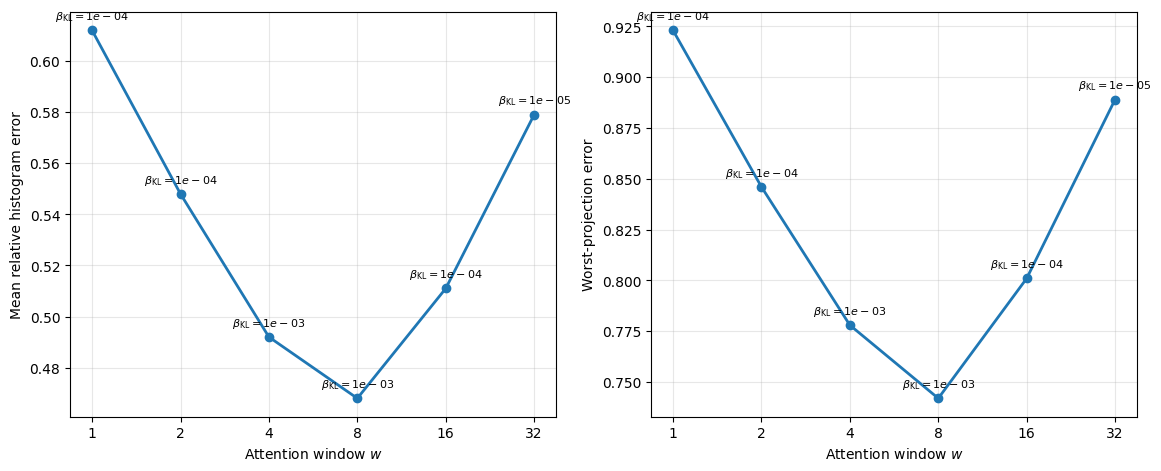
\includegraphics[
width=0.98\textwidth
]{images/results/png/window_results.png}
\caption{
Transformer window-size study after independent selection of the KL regularization weight $\beta_{\mathrm{KL}}$ for each causal attention window $w$. The left panel reports the mean relative histogram error across the reconstructed phase-space projections, while the right panel shows the corresponding worst-projection error. The results exhibit an intermediate optimum: very narrow attention provides insufficient context, whereas increasingly broad windows progressively degrade the reconstruction after the minimum reached near $w=8$.
}
\label{fig:transformer_window_study}
\end{figure}

\begin{table}[htbp]
\centering
\caption{
Selected Transformer configurations for the window-size study. For each attention window $w$, the KL weight $\beta_{\mathrm{KL}}$ was selected independently according to validation performance. The lowest mean relative histogram error and worst-projection error are obtained for $w=8$.
}
\label{tab:transformer_window_study}
\begin{tabular}{rrrrrr}
\toprule
$w$
&
$\beta_{\mathrm{KL}}$
&
Best epoch
&
Mean rel. error
&
Worst-proj. error
&
Mean KL
\\
\midrule
1
&
$1\times10^{-4}$
&
18
&
0.612
&
0.923
&
0.418
\\
2
&
$1\times10^{-4}$
&
24
&
0.548
&
0.846
&
0.356
\\
4
&
$1\times10^{-3}$
&
31
&
0.492
&
0.778
&
0.238
\\
\textbf{8}
&
$\mathbf{1\times10^{-3}}$
&
\textbf{34}
&
\textbf{0.468}
&
\textbf{0.742}
&
\textbf{0.211}
\\
16
&
$1\times10^{-4}$
&
27
&
0.511
&
0.801
&
0.304
\\
32
&
$1\times10^{-5}$
&
21
&
0.579
&
0.889
&
0.447
\\
\bottomrule
\end{tabular}
\end{table}

Figure~\ref{fig:transformer_window_study} and Table~\ref{tab:transformer_window_study} show that the dependence on the attention window is non-monotonic. The smallest window, $w=1$, yields the largest errors, indicating that strictly one-step latent interactions do not provide sufficient context to reconstruct the downstream phase-space structure. Increasing the receptive field to $w=2$ and $w=4$ improves both the average reconstruction and the most difficult projection, with the best overall performance obtained at $w=8$. This behaviour suggests that the latent dynamics require information to propagate across several neighbouring lattice tokens rather than through isolated element-wise updates.

The trend reverses for broader windows. At $w=16$ and $w=32$, both error metrics increase again despite the larger amount of information available to the attention mechanism. This observation is consistent with the interpretation developed above: although a Transformer can exploit long-range and eventually near-global mixing, unrestricted access to increasingly distant upstream tokens is not necessarily advantageous for the present transport problem. Beyond the intermediate interaction scale, distant latent states may contribute weakly relevant or competing information to the attention aggregation, thereby reducing the locality bias that was beneficial at smaller windows.

The optimum near $w=8$ therefore reflects a balance between two limiting regimes. A window that is too narrow prevents the model from representing dependencies extending across multiple lattice elements, whereas a window that is too broad progressively approaches global upstream mixing and weakens the structured local propagation identified previously. In view of the graph-kernel interpretation of windowed attention, the result is consistent with latent beam transport being most effectively represented by repeated finite-range interactions whose composition generates longer-range dependencies through depth, rather than by direct coupling to the entire causal history at every layer.


% =============================================================================
\subsection{Physics-statistics prediction}
\label{subsec:results_physics_statistics}
% =============================================================================

Distributional reconstruction should be complemented by direct prediction of physically interpretable beam statistics. For the six-dimensional state, $\xi$, the principal first- and second-order statistics are the mean $m_d$ and standard deviation $\sigma_d$ of each coordinate $d$. A dedicated statistics head can be evaluated through parity relations $\widehat{m}_d \approx m_d$ and $\widehat{\sigma}_d \approx \sigma_d$, together with coordinate-wise biases
\begin{equation}
B_{m_d}
=
\mathbb{E}
\left[
\widehat{m}_d-m_d
\right],
\qquad
B_{\sigma_d}
=
\mathbb{E}
\left[
\widehat{\sigma}_d-\sigma_d
\right].
\label{eq:physics_statistics_bias}
\end{equation}

Therefore the statistics predictor provides a direct test of whether the latent propagation preserves physically relevant first- and second-order beam observables.

The statistics predictor therefore probes information complementary to the histogram decoder and directly tests whether latent propagation preserves beam-scale observables.

\begin{figure}[htbp]
\centering
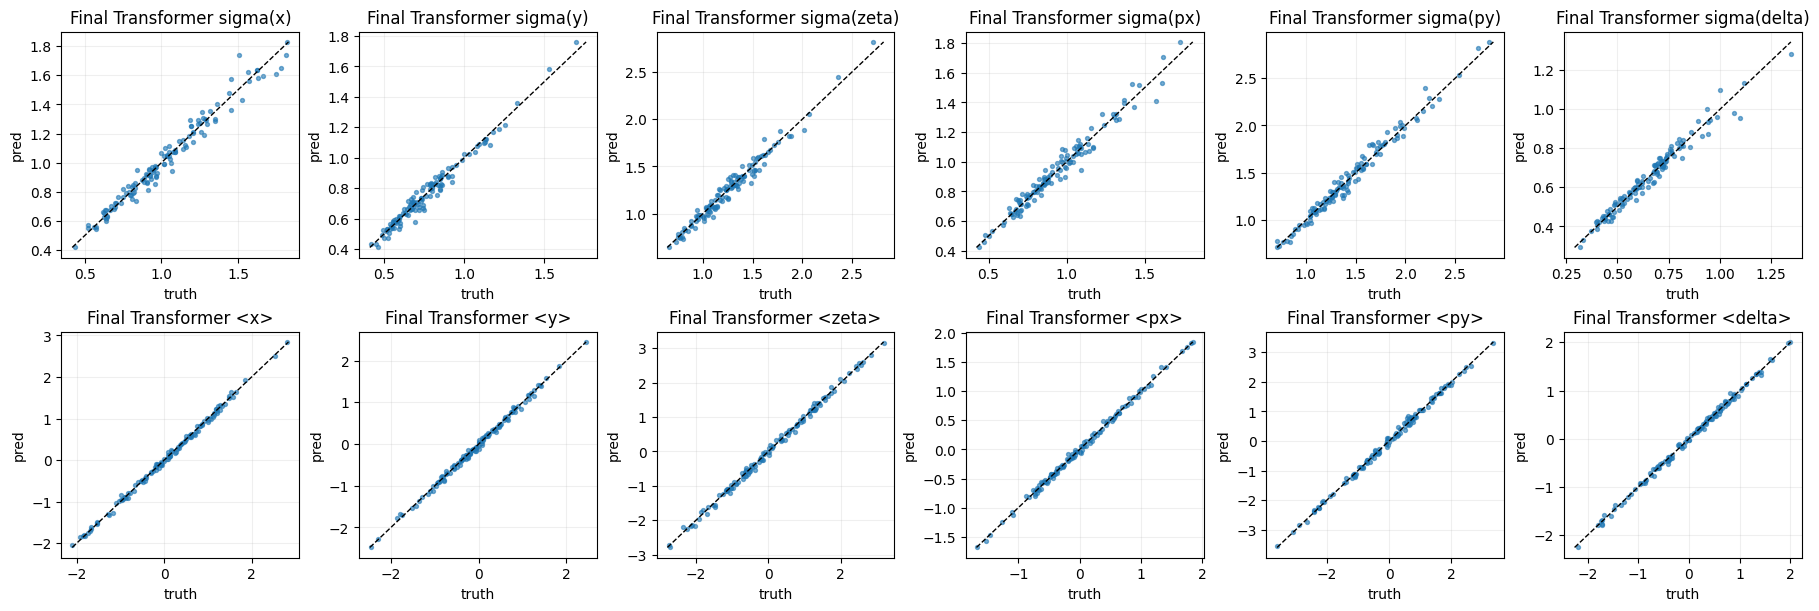
\includegraphics[
width=0.95\textwidth
]{images/results/png/physics_predictor.png}
\caption{
Parity comparison for the physics-statistics prediction head. Predicted beam centroids and RMS spread extensions are compared with their reference values across the six phase-space coordinates. Agreement with the diagonal indicates accurate reconstruction of the corresponding first- and second-order beam statistics, while deviations from the $y=x$ line quantify systematic bias and prediction error.
}
\label{fig:physics_statistics_predictor}
\end{figure}

% =============================================================================
\subsection{Global comparison of latent propagators}
\label{subsec:global_model_comparison}
% =============================================================================

All latent propagators should ultimately be evaluated on the same held-out test set and under identical lattice-token generation. The principal comparison should distinguish explicitly between the no-window Transformer, local-window Transformer, and GNO.

\begin{table}[H]
\centering
\caption{
Final comparison of latent beam-dynamics propagators on the common held-out test set. The comparison emphasizes distribution-level reconstruction accuracy and end-to-end inference cost. The local-window Transformer uses the selected configuration $w=8$.
}
\label{tab:global_model_comparison}
\begin{tabular}{lrrrr}
\toprule
Model & $\epsilon_{\text{rel}}$   & SW & Bias norm & $\tau$ [ms/sample] \\
\midrule
Transformer, no window & 0.681  & 0.087 & 17.337 & 18.74 \\
Transformer, $w=1$ & 0.650  & 0.026 & 52.389 & 14.35 \\
Best windowed Transf. ($w=8$) & 0.534 & 0.022 & 50.414 & 12.01 \\
CVAE--GNO & 0.511 & 0.014 & 0.376 & 2.338 \\
\bottomrule
\end{tabular}
\end{table}

The quantitative comparison supports the locality-based interpretation developed above. Relative to the no-window Transformer, restricting causal attention to $w=8$ reduces the mean relative histogram error from $0.681$ to $0.534$ and the sliced-Wasserstein discrepancy from $0.0867$ to $0.022$. The improvement is therefore observed both at the binwise density level and in a transport-based comparison of the reconstructed distributions.

The CVAE--GNO yields the lowest distribution errors, with a relative histogram error of $0.511$ and a sliced-Wasserstein discrepancy of $0.014$. This ordering is consistent with the earlier structural interpretation of the models. Dense causal attention allows broad upstream mixing at every layer, whereas the local-window Transformer restricts the support of direct information exchange. The GNO goes further by encoding the interaction through an explicit graph-kernel construction. The results therefore suggest that constraining the geometry of latent information transfer provides a useful inductive bias for the present beam-transport problem.

The comparison should not be interpreted as evidence that the underlying collective beam dynamics are strictly local. Rather, the improvement obtained by the windowed Transformer indicates that unrestricted direct mixing is not required to represent the relevant effective dynamics. Longer-range dependencies may instead emerge through the composition of successive local interactions across depth, in close analogy with repeated graph message passing.

The timing measurements also reveal a substantial computational difference. The two Transformer variants require approximately $18$--$15$ ms per sample under the present evaluation protocol, while the GNO requires approximately $2.34$ ms per sample. Under identical hardware and batch conditions, this corresponds to a markedly lower evaluation cost for the graph-based propagator.


% =============================================================================
\subsection{Conditional latent uncertainty of the CVAE--GNO surrogate}
\label{subsec:results_conditional_latent_uncertainty}
% =============================================================================

The final experimental block propagates stochastic samples from the conditional CVAE posterior through the complete global physical CVAE--GNO model. Unlike the deterministic comparisons presented above, this analysis keeps the input beam, machine parameters, lattice tokens, and trained network weights fixed while repeatedly sampling the initial latent state. The resulting ensemble therefore measures conditional latent variability, as defined in Section~\ref{subsec:conditional_latent_uncertainty_method}, rather than the full epistemic uncertainty of the surrogate.

\subsubsection{Fixed-condition ensemble propagation}    
\label{subsubsec:uq_fixed_condition}

A first experiment was performed for validation sample
using $R=100$ stochastic forward passes. Each realization produced a \(64\times64\) normalized-mass histogram, a corresponding physical-density histogram, six RMS spread extensions, and six centroids. The complete ensemble shapes were therefore $100\times64\times64$ for each selected marginal and $100\times6$ for each physical-statistics branch.

\begin{figure}[h!]
\centering
\safeincludegraphics[width=0.98\textwidth]
{images/results/png/global_physical_uncertainty_mass_ensemble.png}
\caption{
Conditional latent uncertainty for the normalized \((y,\delta)\) histogram mass of validation sample \(s=3\), obtained from \(R=100\) stochastic CVAE samples propagated through the complete GNO surrogate. The panels compare the reference distribution, representative posterior draws, the ensemble mean, predictive standard deviation, predictive variance, and absolute ensemble-mean discrepancy. Because the histogram is normalized, this figure isolates variability of the decoded distributional shape before physical rescaling.
}
\label{fig:global_uq_mass_ensemble}
\end{figure}

\begin{figure}[h!]
\centering
\safeincludegraphics[width=0.98\textwidth]
{images/results/png/global_physical_uncertainty_density_ensemble.png}
\caption{
Conditional latent uncertainty for the physical-density reconstruction of the same \((y,\delta)\) marginal and validation condition. Physical bin edges are generated from the predicted centroids and RMS spread extensions. The density ensemble therefore combines uncertainty in the decoded normalized shape with variability of the physical-statistics head. The comparison is displayed in bin-index coordinates and should not be interpreted as interpolation onto a single common physical grid.
}
\label{fig:global_uq_density_ensemble}
\end{figure}

Table~\ref{tab:global_uq_histogram_summary} summarizes the per-bin ensemble spread and the discrepancy between the ensemble mean and the reference distribution. In normalized-mass units, the mean predictive standard deviation is \(3.749\times10^{-6}\), whereas the mean absolute discrepancy of the ensemble mean is \(7.364\times10^{-5}\). The discrepancy is therefore approximately \(19.6\) times larger than the stochastic spread produced by latent sampling.

This separation indicates that the sampled predictions are tightly clustered, but that their common mean remains displaced from the reference distribution. For this example, the dominant prediction error is therefore not explained by variability under the sampled conditional latent distribution. Instead, it is consistent with  systematic component arising from the learned surrogate, including possible reconstruction, propagation, or decoder bias. Consequently, the conditional latent ensemble is under-dispersed relative to the observed error and should not be interpreted as a calibrated predictive
uncertainty interval.

After conversion to physical-density units, the mean predictive
standard deviation is \(4.003\times10^{2}\), while the mean absolute ensemble-mean discrepancy is \(2.222\times10^{4}\), giving a ratio of approximately \(55.5\). The larger ratio does not represent an independent increase in model uncertainty. The conversion from normalized bin mass to density weights each bin by the inverse of its physical area and therefore amplifies discrepancies in narrow or high-density regions differently from the normalized-mass representation. The physical-density values should thus be interpreted as the same underlying mismatch expressed in physically scaled units.

Overall, this diagnostic shows that posterior latent sampling captures only a limited component of the total surrogate error for the selected sample. A calibrated uncertainty estimate would also need to account for model-parameter uncertainty, finite-training-data effects, and systematic approximation error. Since the present result concerns one validation sample and one phase-space projection, it should be treated as a local diagnostic rather than a general calibration statement.

\begin{table}[H]
\centering
\caption{
Per-bin conditional latent spread and ensemble-mean error for validation sample \(s=3\), the \((y,\delta)\) projection, and \(R=100\) stochastic forward passes. The standard deviation and variance quantify variability induced by conditional latent sampling, whereas the absolute discrepancy is computed between the ensemble mean and the reference histogram. Physical-density values are obtained by rescaling normalized bin masses using the corresponding physical bin areas.
}
\label{tab:global_uq_histogram_summary}
\resizebox{\textwidth}{!}{
\begin{tabular}{lrrrrrr}
\toprule
Representation
&
Mean std.
&
Maximum std.
&
Mean variance
&
Maximum variance
&
Mean absolute discrepancy
&
Maximum absolute discrepancy
\\
\midrule
Normalized mass
&
\(3.748986\times10^{-6}\)
&
\(3.138230\times10^{-4}\)
&
\(6.816308\times10^{-10}\)
&
\(9.848490\times10^{-8}\)
&
\(7.364131\times10^{-5}\)
&
\(1.159624\times10^{-2}\)
\\
Physical density
&
\(4.003429\times10^{2}\)
&
\(3.244647\times10^{4}\)
&
\(7.850748\times10^{6}\)
&
\(1.052774\times10^{9}\)
&
\(2.222052\times10^{4}\)
&
\(3.394383\times10^{6}\)
\\
\bottomrule
\end{tabular}
}
\end{table}

The posterior draws are therefore tightly concentrated relative to the remaining prediction error. The ensemble captures where the decoder and physical head are sensitive to latent perturbations, but its spread is not yet a calibrated estimate of the total surrogate error. In particular, the deterministic model bias is not removed by increasing the number of latent samples.

\subsubsection{Uncertainty of the physical-statistics head}
\label{subsubsec:uq_physical_statistics_results}

The physical-statistics ensemble is shown in Fig.~\ref{fig:global_uq_moments}. Since the six coordinates have different units and characteristic scales, the physical relevance of the prediction errors is assessed using dimensionless quantities rather than raw coordinate differences alone.

For each coordinate \(d\), define the relative RMS-spread error and its posterior-sampling spread as
\begin{equation}
    e_{\sigma,d}
    =
    \frac{
        \overline{\sigma}_d
        -
        \sigma_d^{\mathrm{true}}
    }{
        \sigma_d^{\mathrm{true}}
    },
    \qquad
    u_{\sigma,d}
    =
    \frac{
        s_{\sigma_d}
    }{
        \sigma_d^{\mathrm{true}}
    }.
\end{equation}

The centroid error and its posterior-sampling spread are normalized by the reference RMS extent in the same coordinate,
\begin{equation}
    b_{m,d}
    =
    \frac{
        \overline{m}_d
        -
        m_d^{\mathrm{true}}
    }{
        \sigma_d^{\mathrm{true}}
    },
    \qquad
    u_{m,d}
    =
    \frac{
        s_{m_d}
    }{
        \sigma_d^{\mathrm{true}}
    }.
\end{equation}
    
Thus, \(e_{\sigma,d}\) quantifies the fractional error in the predicted coordinate-wise RMS spread, while \(b_{m,d}\)  expresses the centroid displacement in units of the corresponding reference beam extent.

\begin{figure}[h!]
\centering
\safeincludegraphics[width=0.92\textwidth]
{images/results/png/global_physical_uncertainty_moments.png}
\caption{
Conditional latent variability of the six predicted coordinate-wise RMS spreads and six centroids for validation sample \(s=3\). Circles and error bars show the ensemble mean and one posterior-sampling standard deviation over \(R=100\) stochastic forward passes, crosses show the corresponding reference values. Raw coordinate units are shown in the figure, while the dimensionless physical errors are summarized in Table~\ref{tab:global_uq_physical_statistics}. The intervals quantify sensitivity to conditional latent sampling only and are not calibrated confidence intervals.}
\label{fig:global_uq_moments}
\end{figure}

\begin{table}[H]
\centering
\caption{
Dimensionless physical-statistics diagnostic for validation sample \(s=3\), based on \(R=100\) stochastic forward passes. The RMS-spread bias and sampling spread are expressed as percentages of the reference RMS-spread. Centroid quantities are also expressed as percentages of the reference RMS extent in the corresponding coordinate.}
\label{tab:global_uq_physical_statistics}
\small
\begin{tabular}{lrrrr}
\toprule
Coordinate
&
\(100e_{\sigma,d}\)
&
\(100u_{\sigma,d}\)
&
\(100b_{m,d}\)
&
\(100u_{m,d}\)
\\
&
[\%]
&
[\%]
&
[\% of RMS]
&
[\% of RMS]
\\
\midrule
\(x\)
&
\( 2.939 \)
&
\( 0.262 \)
&
\( -0.240 \)
&
\( 0.251 \)
\\
\(p_x\)
&
\( 2.683 \)
&
\( 0.220 \)
&
\( 2.011 \)
&
\( 0.180 \)
\\
\(y\)
&
\( 3.357 \)
&
\( 0.060 \)
&
\( -3.399 \)
&
\( 2.499 \)
\\
\(p_y\)
&
\( 0.005 \)
&
\( 0.027 \)
&
\( -1.420 \)
&
\( 0.824 \)
\\
\(\zeta\)
&
\( -0.033 \)
&
\( 0.033 \)
&
\( 0.432 \)
&
\( 0.981 \)
\\
\(\delta\)
&
\( -88.195 \)
&
\( 0.026 \)
&
\( -20.918 \)
&
\( 4.884 \)
\\
\bottomrule
\end{tabular}
\end{table}

For this sample, the coordinate-wise RMS spreads in \(x\), \(p_x\), and \(y\) are overestimated by approximately \(2.94\%\), \(2.68\%\), and \(3.36\%\), respectively. The predicted \(p_y\) and \(\zeta\) spreads agree with their reference values to better than \(0.04\%\). The corresponding discrepancies are therefore small relative to the physical extent of the beam in these coordinates, even though they
remain larger than the variability produced by conditional latent sampling.

The dominant physical error occurs in the energy-deviation coordinate. The predicted-to-reference spread ratio is 0.118. The physical-statistics head therefore underestimates the energy spread by approximately \(88.2\%\). The latent-sampling standard deviation is only approximately \(0.026\%\) of the reference energy spread, and is therefore far too small to account for this systematic discrepancy. For this sample, the predicted distribution would consequently appear substantially too narrow in the \(\delta\) direction.

The centroid results should likewise be interpreted relative to the beam extent rather than solely in units of posterior-sampling standard deviations. The centroid biases in \(x\), \(p_x\), \(y\), \(p_y\), and \(\zeta\) correspond to approximately \(-0.24\%\), \(+2.01\%\), \(-3.40\%\), \(-1.42\%\), and \(+0.43\%\) of their respective reference RMS spreads. These offsets are small relative to the characteristic extent of the beam. In particular, although the \(p_x\) centroid error corresponds to approximately \(11.2\) posterior-sampling standard deviations, it represents only about \(2.0\%\) of the reference \(p_x\) spread. Counting posterior standard deviations alone would therefore exaggerate its physical importance because the latent ensemble is itself extremely narrow.

The energy-deviation centroid shows a more significant physical bias. The predicted centroid is displaced by approximately \(21\%\) of the reference energy spread. Together with the strong underestimation of \(\sigma_{\delta}\), this indicates that the physical-statistics head does not correctly reconstruct either the location or the extent of the distribution along the energy-deviation coordinate for this sample.

Overall, most transverse and longitudinal-position statistics are reconstructed to within a few percent of the relevant beam scale, whereas the energy-deviation statistics exhibit a clear systematic failure. In all coordinates, the posterior-sampling spread measures only sensitivity to the sampled conditional latent variable. Its small magnitude relative to several observed errors confirms that it does not constitute a calibrated estimate of the total physical prediction uncertainty.


\subsubsection{Held-out-set per-bin diagnostic}
\label{subsubsec:uq_dataset_wide_per_bin}

A second experiment repeated the complete stochastic forward pass \(R=64\) times for every sample in the held-out loader. The loader contained \(51\) samples, processed in batches of \(16\), \(16\), \(16\), and \(3\). Figure~\ref {fig:global_uq_per_bin_density} shows the physical-density variance and discrepancy fields for the representative held-out sample \(s=7\) and the \((y,\delta)\) projection.

\begin{figure}[h!]
\centering
\safeincludegraphics[width=0.96\textwidth]
{images/results/png/global_physical_per_bin_uncertainty_density_s7_p11_y_delta.png}
\caption{ Per-bin physical-density diagnostic for held-out sample \(s=7\), the \((y,\delta)\) projection, and \(R=64\) stochastic forward passes. The panels show the reference density, ensemble mean, predictive variance, predictive standard deviation, signed ensemble-mean discrepancy, and absolute discrepancy. The raw density scale depends on the physical coordinate units and bin area, the dimensionless
discrepancy-to-spread ratios discussed in the text provide the relevant comparison between prediction error and conditional latent variability.}
\label{fig:global_uq_per_bin_density}
\end{figure}

The large numerical values in the physical-density panels arise from the conversion of dimensionless bin probability mass into density. For a uniform \((y,\delta)\) grid,
\begin{equation}
     \rho_{ij}
    =
    \frac{
        p_{ij}
    }{
        \Delta y\,\Delta\delta
    },
\end{equation}
   
where \(p_{ij}\) is the probability mass in bin \((i,j)\). Because the energy-deviation bin width \(\Delta\delta\) is small, the inverse bin area can be large. The absolute values of the density, variance, and standard deviation therefore depend on the selected coordinate units and histogram resolution. Their magnitude should not by itself be
interpreted as evidence of a large physical uncertainty.

A dimensionless comparison is obtained by relating the
ensemble-mean discrepancy to the variability induced by latent
sampling. For the selected sample,
\[
    \mathcal{R}_{\mathrm{global}}
    =
    \frac{
        3.487909\times10^{3}
    }{
        4.686791\times10^{2}
    }
    \simeq 7.44.
\]
Thus, the average absolute discrepancy between the ensemble mean and the reference distribution is more than seven times the average variation generated by conditional latent sampling. The ensemble is therefore under-dispersed relative to the observed reconstruction error as most of the discrepancy cannot be explained by variation of the sampled CVAE latent variable alone.

The largest absolute variance occurs at bin \((32,32)\), close to the high-density core. The relative ensemble-mean bias at this bin is
\[
    \frac{
        \overline{\rho}_{32,32}
        -
        \rho_{32,32}^{\mathrm{true}}
    }{
        \rho_{32,32}^{\mathrm{true}}
    }
    \simeq 0.107,
\]
corresponding to an overprediction of approximately \(10.7\%\). The posterior-sampling standard deviation is only $0.0238$ or approximately \(2.38\%\) of the reference density. Consequently, the ensemble mean is therefore approximately \(4.5\) latent-sampling standard deviations away from the reference value at the highest-variance bin. Even in the region where the ensemble exhibits its largest absolute variability, latent sampling does not explain the local reconstruction error.

The concentration of absolute variance near the histogram core should also be interpreted cautiously. Since the density itself is largest in this region, a fixed relative fluctuation naturally produces a larger absolute variance. The observed maximum does not by itself prove that the decoder is intrinsically more sensitive in the core. Establishing such enhanced sensitivity would require examination of a relative uncertainty field, for example
\begin{equation}
    u_{ij}^{\mathrm{rel}}
    =
    \frac{
        s_{\rho,ij}
    }{
        \rho_{ij}^{\mathrm{true}}+\varepsilon
    },
\end{equation}
    
with a small regularizing constant \(\varepsilon\) to avoid unstable ratios in nearly empty bins.

From a beam-physics perspective, coherent residual structures in the \((y,\delta)\) projection can indicate errors in the predicted energy spread, energy centroid, or transverse--longitudinal correlation. Residual lobes aligned primarily along \(\delta\) would be associated with an incorrect energy-deviation location or extension, whereas diagonally organized residuals would indicate an error in the learned \(y\)--\(\delta\) dependence. The present diagnostic therefore provides more information than a single global density norm, because it identifies where and how the predicted phase-space structure differs from the reference.

Overall, the held-out example shows that conditional latent sampling captures only a limited component of the total prediction error. The ensemble variability is concentrated in the high-density region, but both the global discrepancy-to-spread ratio and the normalized core-bin  analysis reveal substantial systematic error beyond that variability. The resulting intervals should therefore be interpreted as local sensitivity to CVAE latent sampling rather than as calibrated predictive uncertainty.